To reduce the background from $WZ$ and $ZZ$ processes, we veto events
containing an additional lepton satisfying the previously described selection requirements
with $\pt > 10~\GeVc$.

To reject the Drell-Yan background due to the jet energy mismeasurement in 
the recoiling jet, the angle between the dilepton system and the jet in 
the transverse plane must be smaller than 165 degrees. 
This selection is only applied if the jet $\pt>15\GeVc$. 
Figure~\ref{fig:dPhiDiLepJet1_dymc} shows the variable 
$\Delta\phi(\vec{p}_{\ell}, \text{leading jet})$ in data at
the preselection level. The Drell-Yan background is predicted
using the method described in Section \ref{sec:bkg_dy}.

%%%%%%%%
\begin{figure}[!hbtp]
\begin{center}
\label{fig:dphidilepjet_zzpresel}
\subfigure[0-Jet]{\label{subfig:dphidilepjet_0j}
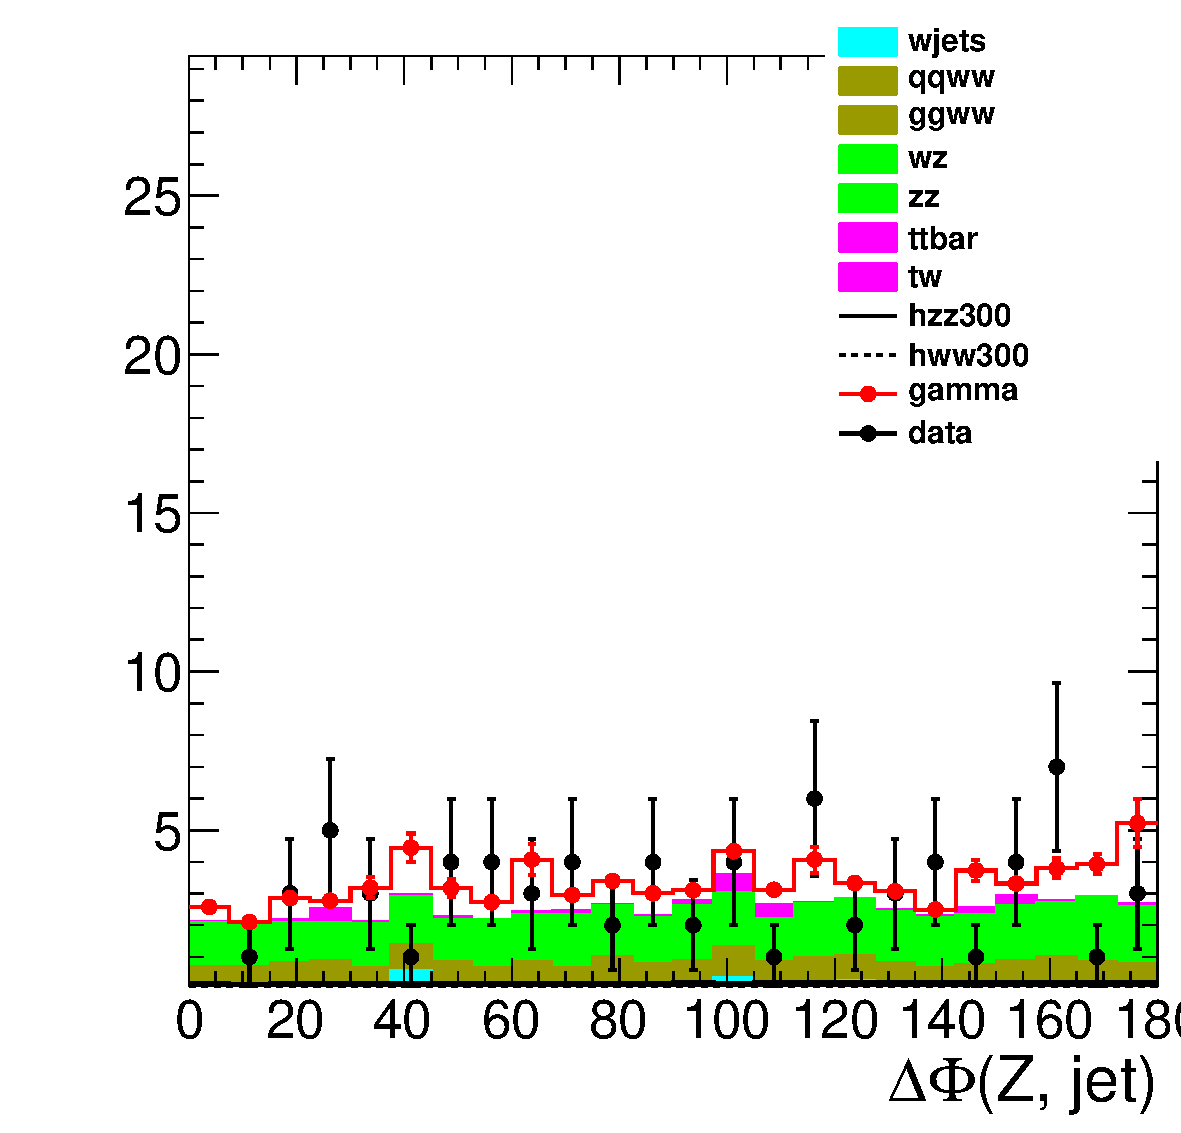
\includegraphics[width=.3\textwidth]{figures/presel_hzz300_dphidilepjet_0j.pdf}}
\subfigure[1-Jet]{\label{subfig:dphidilepjet_1j}
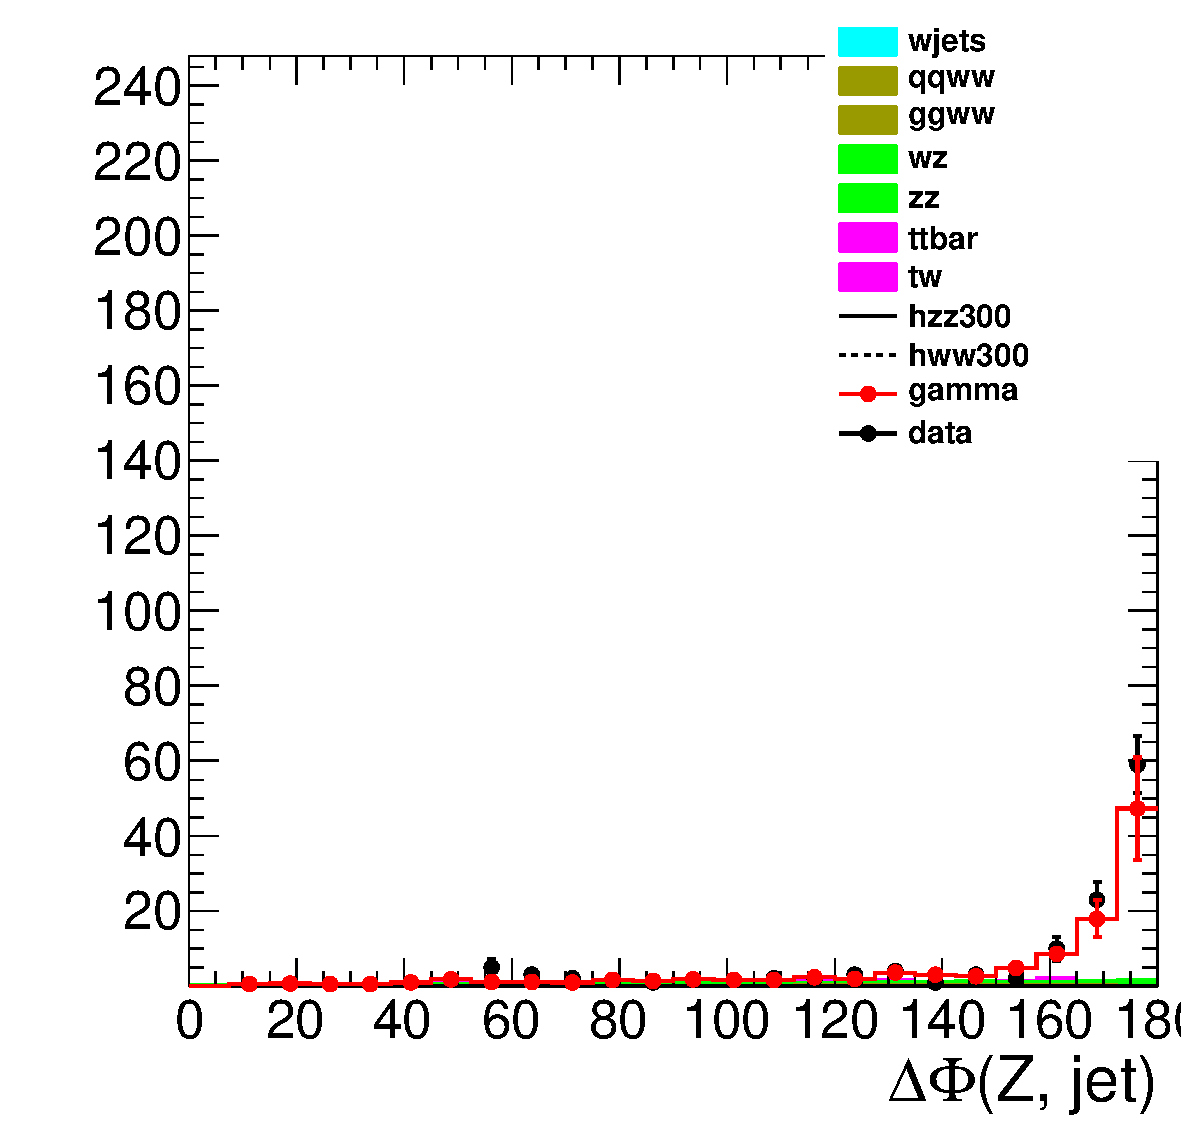
\includegraphics[width=.3\textwidth]{figures/presel_hzz300_dphidilepjet_1j.pdf}}
\subfigure[$\geq$2 Jets]{\label{subfig:dphidilepjet_2j}
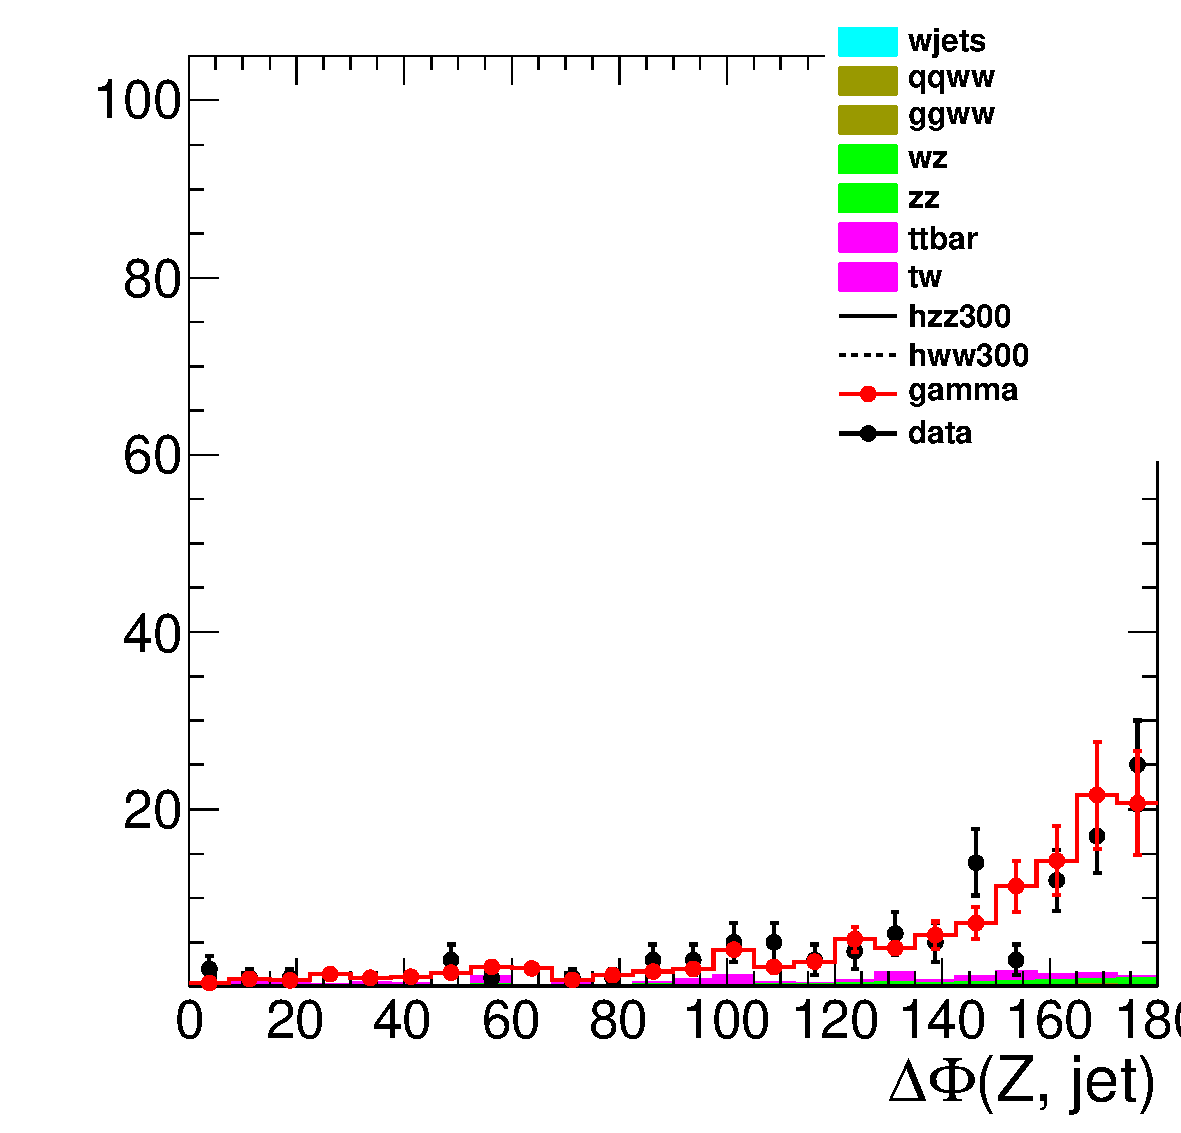
\includegraphics[width=.3\textwidth]{figures/presel_hzz300_dphidilepjet_2j.pdf}}
\caption{$\Delta\phi(\mathrm{dilepton, leading jet})$ distribution after the other $\ZZ$ preselection requirements
corresponding to $1092\pm7$~\ipb data in 0-Jet~\subref{subfig:dphidilepjet_0j}, 1-Jet~\subref{subfig:dphidilepjet_1j}
and 2-Jet~\subref{subfig:dphidilepjet_2j} bins, compared to the expected from simulation for signal and background.
The MC backgrounds are scaled as appropriate and the photon+jets estimate of the Z+jets background is added to the stack.
In the 0-Jet and 1-Jet bins we require this to be less than 165 degrees to reduce the Z+jets background}
\end{center}
\end{figure}
%%%%%%%%

